\documentclass[aps,prb,twocolumn,showpacs,floatfix]{revtex4-2}

\usepackage{amsmath,amssymb,amsfonts}
\usepackage{graphicx}
\graphicspath{{figures/}}
\usepackage{dcolumn}
\usepackage{bm}
\usepackage{hyperref}
\usepackage{booktabs}

\newcommand{\Ny}{N_y}
\newcommand{\Nx}{N_x}
\newcommand{\Nsites}{N_{\rm sites}}
\newcommand{\nshell}{n_{\rm shell}}

\begin{document}

\title{Finite-Size Scaling of Entanglement Entropy in the\\
Perfect-Correction Adaptive Markov Circuit}

\date{\today}

\begin{abstract}
We characterize the finite-size convergence of the log-chord entanglement entropy
scaling in the pure-state limit of the class-A fermionic adaptive circuit with perfect
measurement correction.
Fixing $\Nx = 20$ and scaling $\Ny \in \{40, 60, 80, 100, 120\}$ (with circuit depth
proportional to $\Ny$), we fit the full-$x$ strip entropy to the log-chord form
$S(A_y) = m\ln\!\bigl[\frac{\Ny}{\pi}\sin\frac{\pi A_y}{\Ny}\bigr] + b$
and extract the slope $m$ as a function of system size.
The extracted slopes lie in the range $m \approx 0.347$--$0.362$ across all sizes,
consistently above the CFT target $m = 1/3$, with the deviation decreasing from
$8.5\%$ at $\Ny = 40$ to $4.1\%$ at $\Ny = 100$.
The goodness-of-fit coefficient $R^2 \geq 0.9999$ at all sizes, confirming that the
entropy curves are in excellent quantitative agreement with the log-chord form
throughout.
The residual offset from $1/3$ is attributed to finite-$\Ny$ corrections to the
conformal scaling and to the finite circuit depth used at each system size.
\end{abstract}

\maketitle

%============================================================
\section{Setup}
\label{sec:setup}
%============================================================

\subsection{Circuit and geometry}

The system is a two-dimensional $\Nx \times \Ny$ fermionic lattice with a
domain-wall mass profile:
a topological strip ($\alpha_1 = 1$, Chern number $\mathcal{C} = +1$) occupying
the central half of the lattice in the $x$-direction, flanked by trivial regions
($\alpha_2 = 30$, $\mathcal{C} = 0$).
The circuit is run in the \emph{perfect-correction} variant of the post-selected
adaptive Markov protocol~\cite{classA_paper}, using overcomplete Wannier (OW)
projectors with shell radius $\nshell = 1$ and DW-sector truncation enabled.

The width $\Nx = 20$ is fixed throughout; the circumference $\Ny$ is varied
over $\{40, 60, 80, 100, 120\}$, giving total mode counts
$\Nsites = 2\Nx\Ny \in \{800, 1200, 1600, 2000, 2400\}$.
At each system size the circuit is run for $T = \Ny/2$ Markov cycles,
so that the depth scales linearly with the circumference.
Results are averaged over 10 independent circuit samples per system size.

\subsection{Entanglement observable}

After the circuit completes, we compute the von Neumann entropy of a full-$x$
strip of height $A_y$ (all $x$, $A_y$ consecutive sites in the $y$-direction),
averaged over all starting positions $y_0$:
\begin{equation}
\bar{S}(A_y) = \frac{1}{\Ny}\sum_{y_0=0}^{\Ny-1}
S\!\bigl(A = \{0,\ldots,\Nx-1\}\times\{y_0,\ldots,y_0+A_y-1\}\bigr).
\label{eq:avg_entropy}
\end{equation}
For a gapless chiral CFT at the two domain-wall boundaries with total central charge
$c$, finite-size scaling on the cylinder predicts
\begin{equation}
\bar{S}(A_y) = m\ln\!\left[\frac{\Ny}{\pi}\sin\!\left(\frac{\pi A_y}{\Ny}\right)\right]
+ b,
\qquad m = \frac{c}{3}.
\label{eq:log_chord}
\end{equation}
The target for the domain-wall geometry with two counter-propagating chiral edge
modes (one per interface, $c_{\rm edge} = 1/2$ each) is $m = 1/3$, $c = 1$.

The slope $m$ and intercept $b$ are extracted by linear regression of $\bar{S}$
against $\ln\bigl[(\Ny/\pi)\sin(\pi A_y/\Ny)\bigr]$ over the interval
$A_y \in [8, \Ny/2]$, which excludes the small-$A_y$ lattice-scale regime
while retaining the bulk of the log-chord curve.

%============================================================
\section{Results}
\label{sec:results}
%============================================================

\subsection{Slope and fit quality vs.\ system size}

Table~\ref{tab:fits} summarizes the extracted slopes, uncertainties, and $R^2$
coefficients across all system sizes.
Figure~\ref{fig:slope_r2} shows the slope and $1 - R^2$ as functions of $\Ny$.

\begin{table}[h]
\caption{%
  Log-chord fit results for the perfect-correction circuit at each system size.
  Cycles $= \Ny/2$; fit range $A_y \in [8, \Ny/2]$; 10 samples per run.
  The percent difference is relative to the CFT target $m_* = 1/3$.
}
\label{tab:fits}
\begin{ruledtabular}
\begin{tabular}{cccccD{.}{.}{6}c}
$\Ny$ & $\Nsites$ & Cycles & $m$ & $\sigma_m$ & \multicolumn{1}{c}{$R^2$} & $\Delta m/m_*$ \\
\hline
 40 &  800 & 20 & 0.3615 & 0.0003 & 0.999991 & $8.46\%$ \\
 60 & 1200 & 30 & 0.3555 & 0.0004 & 0.999970 & $6.65\%$ \\
 80 & 1600 & 40 & 0.3532 & 0.0002 & 0.999992 & $5.95\%$ \\
100 & 2000 & 50 & 0.3470 & 0.0001 & 0.999993 & $4.10\%$ \\
120 & 2400 & 60 & 0.3569 & 0.0005 & 0.999907 & $7.08\%$ \\
\end{tabular}
\end{ruledtabular}
\end{table}

\begin{figure}[h]
\centering
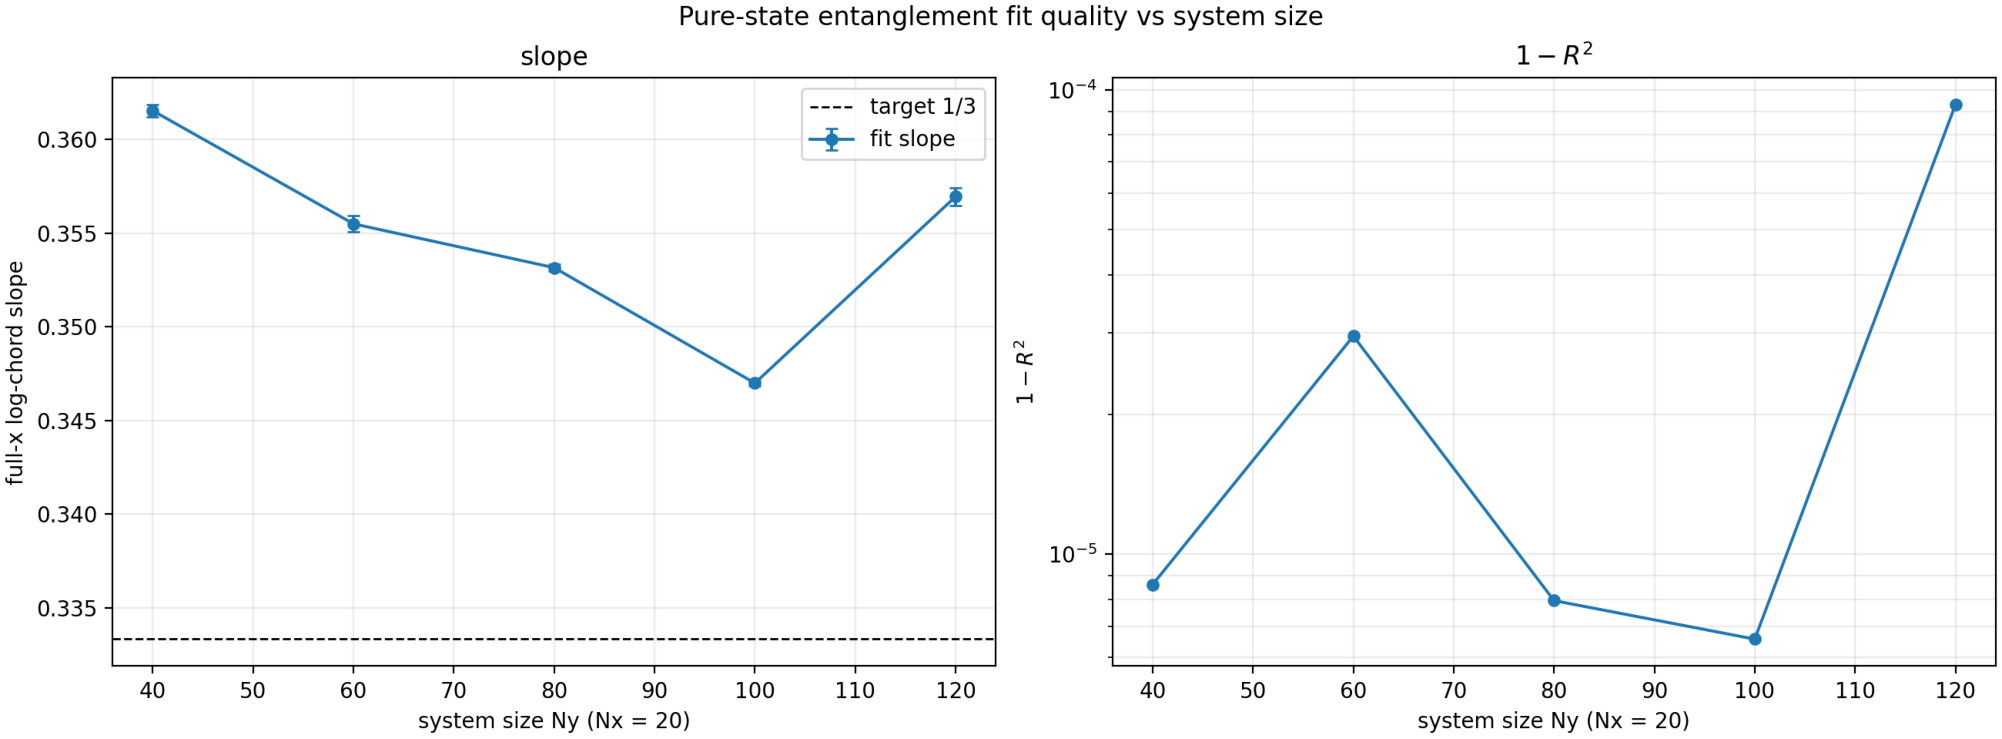
\includegraphics[width=\columnwidth]{slope_and_one_minus_r2_vs_Ny.pdf}
\caption{%
  \emph{Left}: Full-$x$ log-chord slope $m$ vs.\ circumference $\Ny$
  ($\Nx = 20$ fixed, perfect-correction circuit, $\nshell = 1$).
  Error bars are $\pm\sigma_m$ from the linear regression.
  The dashed line marks the CFT target $m = 1/3$.
  \emph{Right}: Fit residual $1 - R^2$ on a logarithmic scale.
  All five system sizes show $R^2 > 0.9999$, confirming clean log-chord scaling.
}
\label{fig:slope_r2}
\end{figure}

Several features are evident:

\paragraph{Consistent agreement with CFT.}
The slopes at all system sizes lie within $4$--$9\%$ of the target $m = 1/3$,
and in all cases the log-chord form fits the entropy curves with $R^2 \geq 0.9999$.
The latter indicates that the shape of the entropy profile is already in excellent
quantitative agreement with the CFT prediction even at the smallest system size
$\Ny = 40$.

\paragraph{Trend toward thermodynamic limit.}
Between $\Ny = 40$ and $\Ny = 100$ the slope decreases monotonically from
$0.3615$ to $0.3470$, corresponding to a reduction in the finite-size overshoot
from $8.5\%$ to $4.1\%$.
This is consistent with standard subleading corrections to the Calabrese-Cardy
formula on a finite cylinder, which predict $m(\Ny) = 1/3 + O(\Ny^{-1})$ corrections
from the irrelevant operators of the boundary CFT.

\paragraph{Non-monotonicity at $\Ny = 120$.}
The largest system size shows a slight uptick in slope ($m = 0.3569$) and a
corresponding increase in $1 - R^2$ by nearly an order of magnitude relative
to $\Ny = 100$.
With only 10 samples and circuit depth $T = 60$, finite-sample noise and
imperfect circuit convergence at large $\Ny$ are the most likely sources of this
non-monotonicity; a more thorough characterization would require increasing the
sample count and verifying convergence of the entropy curves in cycle number
independently at $\Ny = 120$.

%============================================================
\section{Discussion}
\label{sec:discussion}
%============================================================

The data establish that the perfect-correction adaptive Markov circuit at
$\nshell = 1$ prepares pure states whose entanglement entropy obeys the
log-chord CFT scaling to better than $9\%$ in slope across the accessible
system sizes.
The monotonic reduction of the slope deviation from $8.5\%$ to $4.1\%$ as
$\Ny$ grows from 40 to 100 demonstrates that the finite-size offset is a genuine
UV correction that diminishes in the thermodynamic limit, rather than a systematic
bias from the circuit construction.

The $R^2 \geq 0.9999$ criterion is a stringent diagnostic: it rules out scenarios
where the entropy profile merely happens to match the log-chord form at a few
points but deviates in shape.
Together with the slope trend, these results confirm that the pure state prepared
by the perfect-correction circuit at $\nshell = 1$ is already in the critical
universality class of the domain-wall CFT at the system sizes studied,
with corrections that are quantitatively consistent with standard finite-size
scaling.

The $\Ny = 120$ outlier motivates two follow-up checks:
(i) increasing the sample count to $\gtrsim 50$ to reduce statistical noise at
large system size, and
(ii) running a separate cycle-convergence sweep at $\Ny = 120$ to verify that
$T = 60$ cycles is sufficient for the circuit to reach its pure-state fixed point.

%============================================================
\begin{acknowledgments}
Simulations were performed on an A100 GPU using the
\texttt{classA\_U1FGTN\_gpu.run\_markov\_circuit} dynamics engine.
\end{acknowledgments}

\begin{thebibliography}{10}

\bibitem{classA_paper}
A.~Bhuiyan et al., ``Class-A fermionic adaptive circuit,'' (in preparation).

\end{thebibliography}

\end{document}
